\chapter{Introduzione}
In questa introduzione sarà presente una prima parte che andrà a dare le conoscenze di base minime per comprendere cosa sia un sistema operativo e una piccola classificazione di essi, dopodiché seguiranno la descrizione di alcuni concetti che sono fondamentali per comprendere il resto dell'elaborato.

\section{Cos'è un sistema operativo}
Un sistema operativo (SO) è un software che gestisce le risorse hardware e software di un sistema di elaborazione fornendo servizi agli applicativi utente.\\
In un computer quindi esso fornisce l'unica interfaccia diretta con l'hardware e in quanto tale ha un accesso esclusivo con il massimo dei privilegi detto \textit{kernel mode}. Questo comporta che una vulnerabilità all'interno del sistema operativo può portare a gravi conseguenze per l'integrità e la sicurezza del sistema, inoltre qualche malintenzionato potrebbe approfittare di questo bug per trarne profitto.
Uno degli obiettivi principali di un SO è quindi quello di garantire la sicurezza; ulteriore scopo è l'efficienza: un buon sistema operativo deve saper sfruttare al meglio tutte le risorse che ha a disposizione, dalla gestione della memoria per sfruttare al meglio lo spazio alla schedulazione dei processi per ottimizzare i tempi di esecuzione. Come ultimo obiettivo, ma non per questo meno rilevante, deve rendere il più semplice possibile l'utilizzo del dispositivo su cui è installato.
All'interno si un di SO possiamo isolare una specifica parte di codice che è quella che permette al software di interfacciarsi con l'hardware, quindi l'accesso e la gestione delle risorse di un dispositivo. Questa specifica parte si chiama \textit{kernel}, che come suggerisce il nome (nocciolo dall'inglese), rappresenta la parte centrale di un sistema operativo su cui tutto il resto si appoggia.
\newpage

\section{Microkernel e kernel monolitici}
Esistono vari modelli strutturali per i sistemi operativi: monolitici, modulari, a livelli, microkernel ed ibridi. Ad oggi i più diffusi sono gli ibridi, che combinano i vari modelli tra di loro, ma che in gran parte si basano su sistemi monolitici i quali consistono di un unico file binario statico al cui interno sono definite tutte le funzionalità del kernel e che viene eseguito in un unico spazio di indirizzi. Questo comporta dei vantaggi: 
\begin{itemize}
	\item[-] efficienza:  motivo principale per cui la maggior parte dei sistemi operativi ancora oggi si basano su kernel in gran parte monolitici, lavorando nello stesso spazio di indirizzi e gestendo tutto attraverso chiamate a procedura il SO risulterà molto reattivo e performante;
	\item[-] semplicità: in quanto non ha una vera e  propria strutturazione, bensì il codice è tutto in un unico file binario, risulta chiaramente più semplice da progettare anche se poi l'implementazione risulta difficile.
\end{itemize} 
D'altra parte ha anche degli svantaggi: 
\begin{itemize}
	\item[-] inserimento di un nuovo servizi: questo richiede la ricompilazione del kernel, quindi non permette l'inserimento di un nuovo servizio a runtime (problema risolto nei modelli ibridi);
	\item[-] dimensione: dovendo gestire tutte le principali funzionalità del sistema operativo, il kernel sarà composto da milioni di righe di codice sorgente (MSLOC - linux ha circa 20MSLOC) e questo porta direttamente al successivo grosso svantaggio;
	\item[-] sicurezza: maggiore è il numero di righe di codice maggiore sarà il numero di possibili bug; essendo tutto il codice eseguito nello stesso spazio di indirizzi un bug rischia di far bloccare l'intero sistema anche se il problema è molto piccolo e isolato a una minima funzione del kernel.
\end{itemize}
All'estremo opposto troviamo i \textit{microkernel} che sono composti da un kernel ridotto al minimo indispensabile, che comprende la gestione della memoria, dei processi e della CPU, le comunicazioni tra processi (IPC) e l'hardware di basso livello, mentre tutto il resto deve essere gestito da server (daemon) che operano sopra al kernel, quindi in spazi di indirizzi separati.\\ I microkernel sono spesso usati in sistemi embedded, in applicazioni mission critical di automazione robotica o di medicina, a causa del fatto che i componenti del sistema risiedono in aree di memoria separate, private e protette \cite{kernelWikipedia}.\\
Anche questo modello ha dei vantaggi:
\begin{itemize}
	\item[-] flessibilità: l'inserimento di un nuovo servizio avviene al di sopra del kernel quindi in qualsiasi momento è possibile aggiungere o togliere servizi senza dover modificare il kernel;
	\item[-] sicurezza: minore quantità di codice eseguita in kernel mode (quindi minore quantità di bug e minore superficie attaccabile) quindi maggiore sicurezza del sistema; inoltre i servizi lavorano in uno spazio di indirizzi differente da quello del kernel di conseguenza se un server (su cui viene eseguito un servizio) smette di funzionare tutto il resto del sistema continua a funzionare normalmente e si potrà procedere a riavviare quel singolo servizio;
	\item[-] semplicità: essendo il codice composto da qualche decina di migliaia di righe di codice (KSLOC) risulta molto più facile da scrivere.
\end{itemize}
Dall'altro lato ha un grande svantaggio:
\begin{itemize}
	\item[-] efficienza: dato che ogni servizio è eseguito a livello utente, l'utilizzo di uno qualsiasi di questi richiede il ricorso a chiamate di sistema che rallentano fortemente l'esecuzione di ogni operazione, motivo principale per cui ancora oggi i sistemi operativi si basano in gran parte su sistemi monolitici.
\end{itemize}
In Figura~\ref{fig:MonolithicVSmicrokernel} si possono vedere in maniera schematica le differenza tra kernel monolitici e mircrokernel.

\begin{figure}[h]
  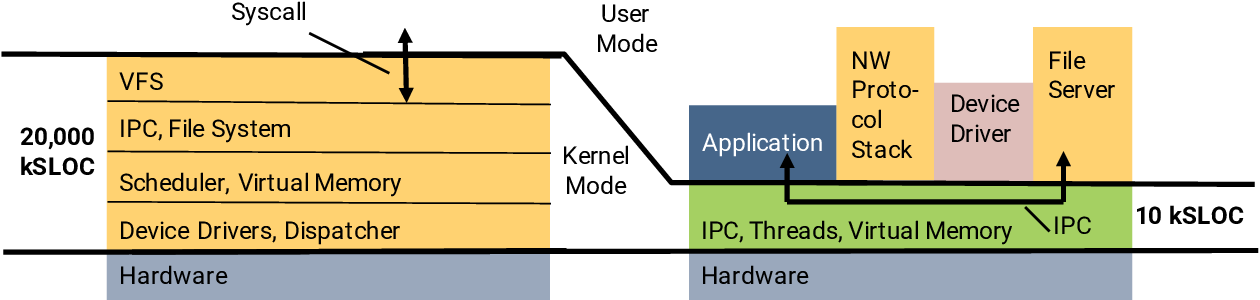
\includegraphics[width=\linewidth]{img/MonolithicVSmicrokernel.png}
  \caption{Kernel monolitici (sinistra) VS Microkernel (destra)}
  \label{fig:MonolithicVSmicrokernel}
\end{figure}
\newpage

\section{Scheduling}
Solitamente con il solo termine scheduling si intende quello a breve termine della CPU, cioè la funzionalità che determina quale tra i processi (thread) in attesa della CPU la otterranno. Ci sono vari metodi che si differenziano per modalità e prestazioni. Gli algoritmi che traducono questi metodi si chiamano politiche di scheduling.
Una particolare politica di scheduling rilevante per questo testo è Round Robin o scheduling circolare: consiste nel determinare un quanto di tempo (time slice) nella quale i processi ottengono la CPU. Una volta esaurito questo tempo il processo viene interrotto e inserito in fondo alla coda dei pronti. In questo modo tutti i processi ottengono la CPU per un tempo massimo stabilito; inoltre è possibile stabilire il tempo di attesa prima dell'esecuzione di ciascun processo in base al numero di processi che lo precedono.

\section{Hypervisor}
Un \textit{hypervisor}, chiamato anche virtual machine monitor (VMM), è un tipo di sotware/firmware che permette di creare ed eseguire macchine virtuali. Un computer sul quale un hypervisor esegue una o più macchine virtuali prende il nome di \textit{host machine}, mentre le singole macchina virtuali prendono il nome di \textit{guest machine}. Su ognuna è possibile eseguire un sistema operativo (anche diverso) che eseguirà la maggior parte delle istruzioni direttamente sulle risorse hardware virtualizzate rese disponibili dall'hypervisor.